%! TEX root = **/000-main.tex
% vim: spell spelllang=en:

\section{Normalized arc sine kernel on the Frénay datasets}
\sectionmark{Norm. arcsine kernel}

\Cref{fig:mse-frenay-original} shows the results obtained by
\textcite{frenayParameterinsensitiveKernelExtreme2011} for the arc-sine kernel
on the different datasets. These plots are generated using the table of results
from the original paper. The shaded area corresponds to the 95\% confidence
interval provided by the authors. The horizontal red line corresponds to the RBF kernel and
the dotted lines above and below are the 95\% confidence interval for the RBF.
Note that the table had 2 significant digits, and in \texttt{Elevators} dataset, the
lower bound of the confidence interval for the RBF is equal to the mean value,
so it is overlapping in the plot.

\begin{figure}[H]
    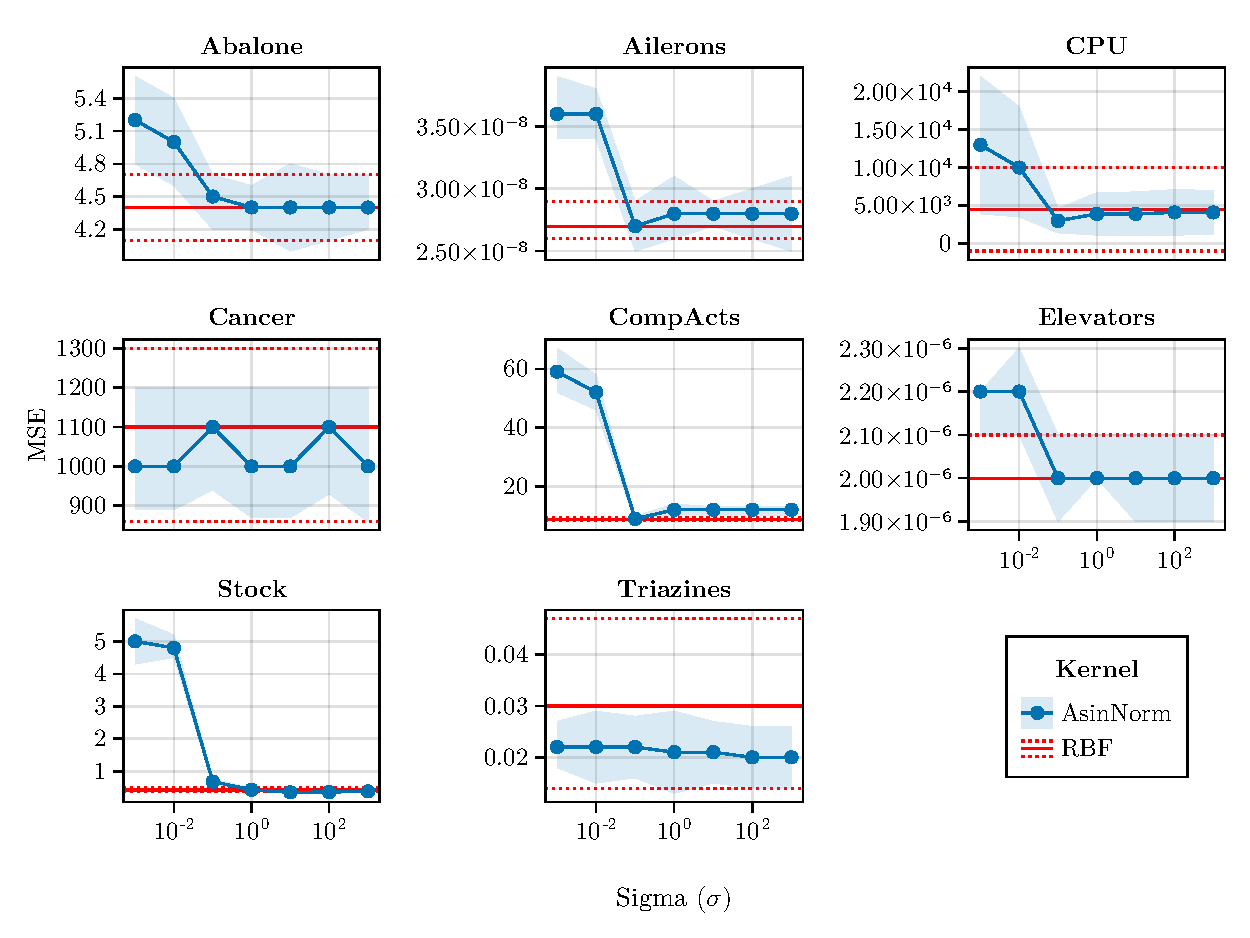
\includegraphics[width=.7\textwidth]{plots/MSE_frenay_original}
    \caption{MSE from \cite{frenayParameterinsensitiveKernelExtreme2011}}
    \label{fig:mse-frenay-original}
\end{figure}

\begin{figure}[H]
    % TODO: make color more clear
    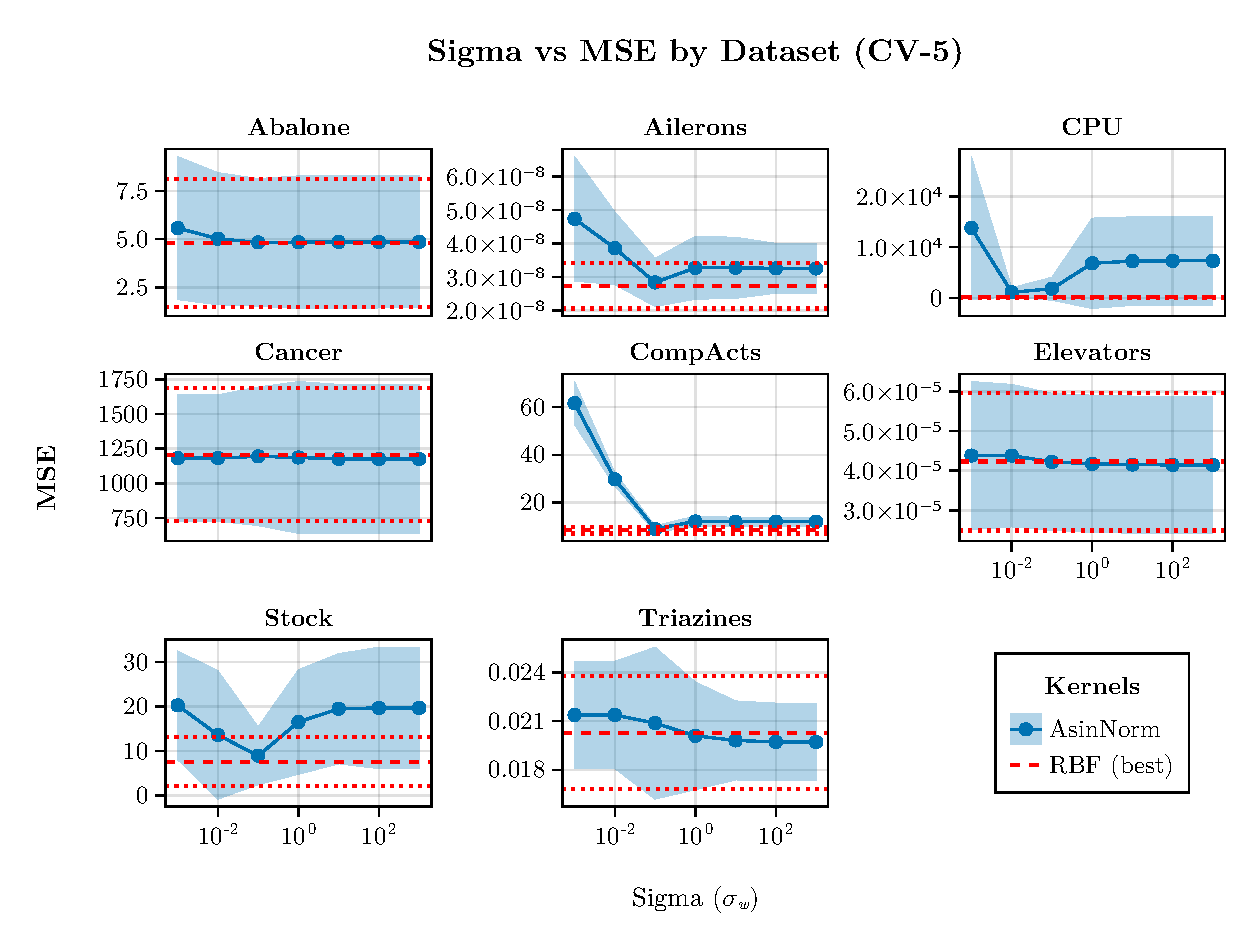
\includegraphics[width=.7\textwidth]{plots/MSE_frenay}
    \caption{Our reproduction of the results from \cite{frenayParameterinsensitiveKernelExtreme2011}}
    \label{fig:mse-frenay}
\end{figure}

\Cref{fig:mse-frenay} shows the results of the arc-sine
kernel~(normalized and non-normalized) on the same datasets used by \textcite{frenayParameterinsensitiveKernelExtreme2011}. The shading corresponds to the standard deviation when averaging the
cross-validation results.

% TODO: plots side by side so it's easier to compare
When comparing \cref{fig:mse-frenay-original} and \cref{fig:mse-frenay}, we
can see that the results are similar, but there are notable differences in some
datasets. In general, the confidence intervals are larger in our results, which
is expected since we use a different resampling method.

\begin{description}
    \item[\texttt{Abalone}] Our confidence interval is much larger and ecompases
        their whole confidence interval. Our results do not show significant difference
        for lower values of sigma as theirs does, but there is an appreciable
        difference for $\sigma_w=10^{-3}$.
    \item[\texttt{Ailerons}] The results are consistent with the original paper.
    \item[\texttt{CPU}] The behaviour is similar. The confidence interval of RBF
        is much tighter in our results.
    \item[\texttt{Cancer}] Similar to the original paper, but again the confidence
        interval of our results is significantly larger.
    \item[\texttt{CompActs}] In this case, the results are extremely similar.
    \item[\texttt{Elevators}] Our results do not exhibit the same behaviour and
        are 1 order of magnitude higher than theirs in both arc-sine and RBF. Looking
        at results on the dataset in OpenML\footnote{\url{https://www.openml.org/search?type=data&sort=runs&id=216&status=active}}, other people obtain values of RMSE between $0.0067$ and $0.0046$ which
        in MSE is between $0.000045$ and $0.000022$. These results align with ours,
        so there may be a typo in the original paper or there are using a different
        version of the dataset or some other difference in the preprocessing.
    \item[\texttt{Stock}] For this dataset, the behaviour is very different. The
        stock dataset consists of stock data from 10 companies.
    \item[\texttt{Triazines}] The behaviour is similar. As in \texttt{CPU},
        the confidence interval of RBF is much tighter in our results.
\end{description}

The datasets where the results are significantly different are \texttt{Elevators}
and \texttt{Stock}. In the case of \texttt{Elevators}, we have already discussed
that there may be some difference in the preprocessing of the dataset.

% TODO: Is this a correct interpretation?
\texttt{Stock} is a dataset of daily stock data from 10 companies. This
means that the data is not independent, and thus the resampling method used
by \textcite{frenayParameterinsensitiveKernelExtreme2011} which takes
90\% of the data for training and 10\% for testing may not be appropriate. Since
there is a high probability that the test set contains data from days that are
adjacent to the training set. Our resampling method, which uses random
50\% splits is not affected as much by this problem and thus our results are
different.
